

\section{Langage Python}

\begin{frame}{Comment faire du data mining en pratique ?}

    \begin{itemize}
        \item<+-> \textbf{Python} : langage versatile avec bibliothèques puissantes (pandas, scikit-learn, numpy)
        \item<+-> \textbf{R} : langage statistique avec écosystème riche pour l'analyse
        \item<+-> \textbf{SQL} : interrogation et manipulation de bases de données
        \item<+-> \textbf{Spark} : traitement distribué de grands volumes de données
        \item<+-> \textbf{Tableau, Power BI} : visualisation et exploration interactive
    \end{itemize}
\end{frame}





    \begin{frame}[fragile]{Quelques rappels : variables et types}
        \begin{itemize}
        \item<+->[\textcolor{white}{a}] La syntaxe de Python repose sur une série d'instructions et des mots clés bien précis
\begin{lstlisting}[language=Python, morekeywords={as, TypeError}, numbers=none]
a = 1
print(a) # affiche 1
\end{lstlisting}
        \item<+-> \texttt{a} est une \textbf{variable} et 1 est sa \textbf{valeur}
        \item<+-> la variable \texttt{a} a un type
\begin{lstlisting}[language=Python, morekeywords={as, TypeError}, numbers=none]
print(type(a)) # affiche 'int'
\end{lstlisting}
        \end{itemize}
  \end{frame}
  


  \begin{frame}[fragile]{Quelques rappels : variables et types}
    \begin{itemize}
    \item<+->[\textcolor{white}{a}] La syntaxe de Python repose sur une série d'instructions et des mots clés bien précis
\begin{lstlisting}[language=Python, morekeywords={as, TypeError}, numbers=none]
a = 3.14
print(a) # affiche 3.14
\end{lstlisting}
    \item \texttt{a} est une \textbf{variable} et 3.14 est sa \textbf{valeur}
    \item la variable \texttt{a} a un type
\begin{lstlisting}[language=Python, morekeywords={as, TypeError}, numbers=none]
print(type(a)) # affiche 'float'
\end{lstlisting}
    \end{itemize}
\end{frame}



\begin{frame}[fragile]{Quelques rappels : variables et types}
    \begin{itemize}
    \item<+->[\textcolor{white}{a}] La syntaxe de Python repose sur une série d'instructions et des mots clés bien précis
\begin{lstlisting}[language=Python, morekeywords={as, TypeError}, numbers=none]
a = "python"
print(a) # affiche "python"
\end{lstlisting}
    \item \texttt{a} est une \textbf{variable} et \texttt{"python"} est sa \textbf{valeur}
    \item la variable \texttt{a} a un type
\begin{lstlisting}[language=Python, morekeywords={as, TypeError}, numbers=none]
print(type(a)) # affiche 'str'
\end{lstlisting}
    \end{itemize}
\end{frame}


\begin{frame}[fragile]{Quelques rappels : variables et types}
    \begin{itemize}
    \item<+->[\textcolor{white}{a}] La syntaxe de Python repose sur une série d'instructions et des mots clés bien précis
\begin{lstlisting}[language=Python, morekeywords={as, TypeError}, numbers=none]
a = [1, 2, 3]
print(a) # affiche [1, 2, 3]
\end{lstlisting}
    \item \texttt{a} est une \textbf{variable} et [1, 2, 3] est sa \textbf{valeur}
    \item la variable \texttt{a} a un type
\begin{lstlisting}[language=Python, morekeywords={as, TypeError}, numbers=none]
print(type(a)) # affiche 'list'
\end{lstlisting}
    \end{itemize}
\end{frame}


    \begin{frame}[fragile]{Quelques rappels : variables et types}
        \begin{block}{Opérations mathématiques}
        \medskip
        Les opérations mathématiques sont définies en python pour les types numériques (entiers, réels).\\
        Certaines le sont aussi pour les \textbf{chaînes de caractères}
        \end{block}
        
\begin{lstlisting}[language=Python, morekeywords={as}, numbers=none]
5 + 4 # donne 9
"He" + "llo" # donne "Hello"
"Hello" * 2 # donne "HelloHello"
\end{lstlisting}
    \end{frame}
  
  \begin{frame}[fragile]{Quelques rappels : syntaxte}
  
    \begin{block}{Syntaxe en blocs indentés}
        \begin{itemize}
        \item Indentation : décalage de lignes de code
        \item Délimiter des blocs logiques
        \end{itemize}
    \end{block}
  
    \bigskip

\begin{lstlisting}[language=bash, morekeywords={def, list}, numbers=none]
dice = [1, 2, 3, 4, 5, 6]
value = random.choice(dice)
if value == 6:
    print(value, "You won!")
else:
    print(value, "Try again!")
\end{lstlisting}

\end{frame}










\begin{frame}[fragile]{Fonctions}
    
    \begin{block}{Définition}
        \medskip
        Une fonction est une portion du code qui effectue une tâche précise. Elle permet
        \begin{itemize}
            \item de structurer le code 
            \item d'éviter de dupliquer des parties du code, de simplifier la lecture
        \end{itemize}
    \end{block}
  
    \begin{overprint}
      
      \onslide<1>
\begin{lstlisting}[language=Python, morekeywords={}, numbers=none]
def fct(a, b, c):
    d = (a + b) * c
    return d


fct(1, 2, 3)
fct("py", "thon", 3)
\end{lstlisting}
  
    \onslide<2>
\begin{lstlisting}[language=Python, morekeywords={}, numbers=none]
def fct(a=1, b=1, c=1):
    d = (a + b) * c
    return d

fct()
fct(1, 2, 3)
fct("py", "thon", 3)
\end{lstlisting}

    \onslide<3>
\begin{lstlisting}[language=Python, morekeywords={}, numbers=none]
def play():
    dice = [1, 2, 3, 4, 5, 6]
    value = random.choice(dice)
    if value == 6:
        print(value, "You won!")
    else:
        print(value, "Try again!")

play()
play()
play()
\end{lstlisting}
    \end{overprint}

  \end{frame}


\begin{frame}[fragile]{Modules et imports}
    \begin{block}{Modules}
        \medskip
        Python est structuré en un ensemble de modules correspondant à des \textcolor{red}{tâches spécifiques}
        \begin{itemize}
            \item \texttt{random} : simulation aléatoire
            \item \texttt{matplotlib} : visualisation de données
            \item \texttt{nltk, spacy} : analyse textuelle
        \end{itemize}
    \end{block}

    \onslide<2>
    \begin{columns}
        \begin{column}{.4\textwidth}
            \begin{block}{Dans chaque module}
                \medskip
                \begin{itemize}
                    \item d'autres modules
                    \item des fonctions
                \end{itemize}
            \end{block}
        \end{column}

        \begin{column}{.6\textwidth}
\begin{lstlisting}[language=Python, morekeywords={}, numbers=none]
import random
random.choice([1, 2, 3, 4, 5, 6])
\end{lstlisting}
        \end{column}
    \end{columns}


\end{frame}


\begin{frame}{Modules NLTK et SpaCy}
    NLTK et SpaCy sont deux boites à outils pour l'analyse textuelle.

    Large éventail de fonctionnalités : tokenization, lemmatization, mots clés, etc.
    
    \bigskip

    \footnotesize
    \centering
    \begin{tabular}{|l|l|l|}
        \hline
        \textbf{Aspect}                 & \textbf{NLTK}                           & \textbf{SpaCy}                         \\
        \hline
        \textbf{Objectif principal}     & Exploration     & Production       \\
        \hline
        \textbf{Facilité} & Simple & Simple               \\
        \hline
        \textbf{Performances}           & Plus lent            & Optimisé pour la vitesse                 \\
        \hline
        \textbf{Fonctionnalités} & Moins avancé     & Modèles pré-entraînés        \\
        \textbf{modernes} &      & contextuels        \\
        \hline
        \textbf{Modèles pré-entraînés}  & Implémentation manuelle & Intégrés et faciles d’accès             \\
        \hline
    \end{tabular}
        
\end{frame}

\begin{frame}{Quid des LLM ?}
    \centering
    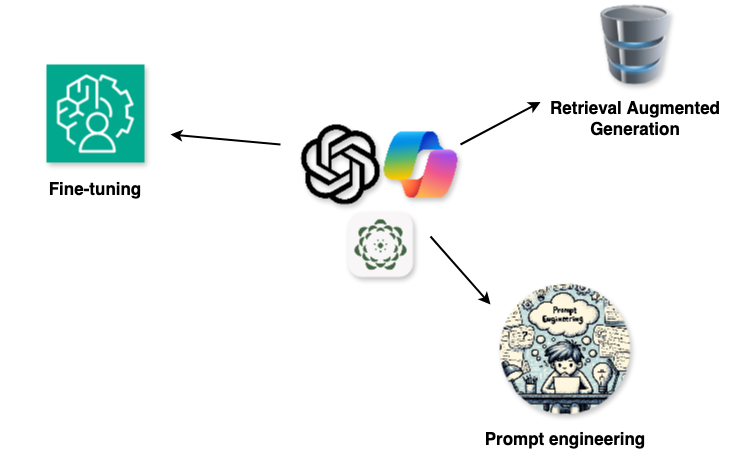
\includegraphics[width=\textwidth]{img/rag-fine-prompt.png}
\end{frame}
